\documentclass[12pt]{article}

\usepackage[utf8]{inputenc}
\usepackage{latexsym,amsfonts,amssymb,amsthm,amsmath}
\usepackage{tikz}
\usepackage{stanli}
\usetikzlibrary{shapes,calc,through,3d,patterns}
\usetikzlibrary{arrows.meta,decorations.pathreplacing,angles,quotes}
\usepackage{multicol}
\usepackage{geometry}
\usepackage{mathtools}
\usepackage{siunitx}
\usepackage{booktabs}

\setlength{\parindent}{0in}
\setlength{\oddsidemargin}{-0.25in}
\setlength{\textwidth}{7in}
\setlength{\textheight}{9.3in}
\setlength{\topmargin}{-1in}
\setlength{\headheight}{18pt}

\newcommand\blfootnote[1]{%
    \begingroup
    \renewcommand\thefootnote{}\footnote{#1}%
    \addtocounter{footnote}{-1}%
    \endgroup
}

\definecolor{darkred}{rgb}{0.6,0,0}

\newcommand{\bolddelta}{\boldsymbol\delta}
\newcommand{\boldxi}{\boldsymbol\xi}

\begin{document}

\noindent ME473 - Dynamic finite element analysis of structures\hfill EPFL\\
Stefano Burzio \hfill 2025\\
\vspace{0.3cm}

\hspace*{\fill}\textbf{\Large Problem set 7}\hspace*{\fill}

\hrulefill

\subsection*{Problem 1}
Consider the shape functions for the AMC element:
$$ {}^a\mathbf  h_i(\boldxi) =\begin{bmatrix}
        (1 + \xi_1^i \xi_1)(1 + \xi_2^i \xi_2)(2 + \xi_1^i \xi_1 + \xi_2^i \xi_2 - \xi_1^2 - \xi_2^2)/8 \\
        b(1 + \xi_1^i \xi_1)(\xi_2^i + \xi_2)(\xi_2^2 - 1)/8                                            \\
        -a(\xi_1^i + \xi_1)(\xi_1^2 - 1)(1 + \xi_2^i \xi_2)/8
    \end{bmatrix}^T$$
where $\boldxi^i=\{\xi_1^i,\xi_2^i\}^T$ are the local coordinates of node $i=1,\dots,4$.
\begin{center}
    \begin{tikzpicture}[scale=2.5]
        % \draw[step=1.0,black,thin] (-2,0) grid (4,4);
        \draw[fill=gray!40,thick] (-1.5,0.5) -- (-0.5,0.5) -- (-0.5,1.5) -- (-1.5,1.5) -- cycle;
        \draw[thick] (-1.5,0.5) -- (-0.5,0.5) -- (-0.5,1.5) -- (-1.5,1.5) -- cycle;
        \draw[ultra thin,-latex] (-1.8,1) -- (-0.2,1) node[right]{$\xi_1$};
        \draw[ultra thin,-latex] (-1,0.2) -- (-1,1.8) node[above]{$\xi_2$};
        \node[,draw,shape=circle,fill=white,minimum size=2mm,line width=0.3mm,inner sep=0] at (-1.5,0.5) {};
        \node[,draw,shape=circle,fill=white,minimum size=2mm,line width=0.3mm,inner sep=0] at (-0.5,0.5) {};
        \node[,draw,shape=circle,fill=white,minimum size=2mm,line width=0.3mm,inner sep=0] at (-0.5,1.5) {};
        \node[,draw,shape=circle,fill=white,minimum size=2mm,line width=0.3mm,inner sep=0] at (-1.5,1.5) {};
        \node[below left] at (-1.5,0.5) {$1$};
        \node[above left] at (-1.5,1.5) {$4$};
        \node[below right] at (-0.5,0.5) {$2$};
        \node[above right] at (-0.5,1.5) {$3$};
        \draw[ultra thin] (-0.5,1.2) -- (0,1.4) node[right]{\small Side 2-3  ($\xi_1=1$)};
    \end{tikzpicture}
\end{center}
\begin{itemize}
    \item[a)] Show that, for $i,j=1,\dots 4$, the Kronecker delta property holds: $${}^a\mathbf  h_i(\boldxi^j)=\begin{bmatrix}
                  \delta_{ij} \\ 0 \\ 0
              \end{bmatrix}^T$$
          where $\delta_{ij}$ is the Kronecker symbol.
    \item[b)] Show that the generalized displacement function defined by
          $$ {}^eu_3^h(\boldxi,t)  =\sum_{i=1}^4  {}^a\mathbf h_i(\boldxi) \begin{bmatrix}
                  {}^ed^i(t) \\[2pt] {}^e{\theta}^i_1(t) \\[2pt] {}^e{\theta}^i_2(t)
              \end{bmatrix}= {}^a\mathbf{H}(\boldxi){}^e\mathbf{q}(t)$$
          is a non-conforming one by evaluating $u_3^h$, $\theta_1^h$ and $\theta_2^h$ on the side 2-3 ($\xi_1=1$) and by showing that $\theta_2^h$ could be discontinuous along this edge.
\end{itemize}

\subsection*{Problem 2}
Demonstrate that, in the AMC plate bending element, selecting a displacement function that includes the quartic terms $x^4$ and $y^4$ instead of the mixed cubic terms $x^3 y$ and $x y^3$ results in displacement discontinuities along the element boundaries.

\subsection*{Problem 3}
Consider the following shape functions:
$$ {}^a\mathbf  h_i(\boldxi) =\begin{bmatrix}
        f_i(\xi_1)f_i(\xi_2)     \\
        bf_i(\xi_1)g_i(\xi_2 )   \\
        -a g_i(\xi_1)f_i(\xi_2 ) \\
    \end{bmatrix}^T$$
where $\boldxi^i=\{\xi_1^i,\xi_2^i\}^T$ are the local coordinates of node $i=1,\dots,4$ and $f_i$ and $g_i$ are the Hermite cubic shape functions:
\begin{align*}
    f_i(\xi) & =(-\xi^i\xi^3+3\xi^i\xi+2)/4, & g_i(\xi) & =(\xi^3+\xi^i\xi^2-\xi-\xi^i)/4.
\end{align*}
Show that the generalized displacement function, defined by
$$ {}^eu_3^h(\boldxi,t)  =\sum_{i=1}^4  {}^a\mathbf h_i(\boldxi) \begin{bmatrix}
        {}^ed^i(t) \\[2pt] {}^e{\theta}^i_1(t) \\[2pt] {}^e{\theta}^i_2(t)
    \end{bmatrix}= {}^a\mathbf{H}(\boldxi){}^e\mathbf{q}(t),$$
has twist $\frac{\partial^2}{\partial\xi_1\partial\xi_2}{}^eu_3^h$ zero at the four nodal points.








\end{document}